\chapter{Постановка задачи}
\label{sec:Chapter1} \index{Chapter1}

	Согласно мировым стандартам, качество РЛИ измеряется по отклику от уголковых отражателей или от транспондеров. Данные калибровочные объекты ещё называют точечными целями, то есть одиночными, изолированными рассеивателями. Пример такого отклика представлен на рисунке \ref{fig:point_target}.
	
\begin{figure}[ht]
    \centering
    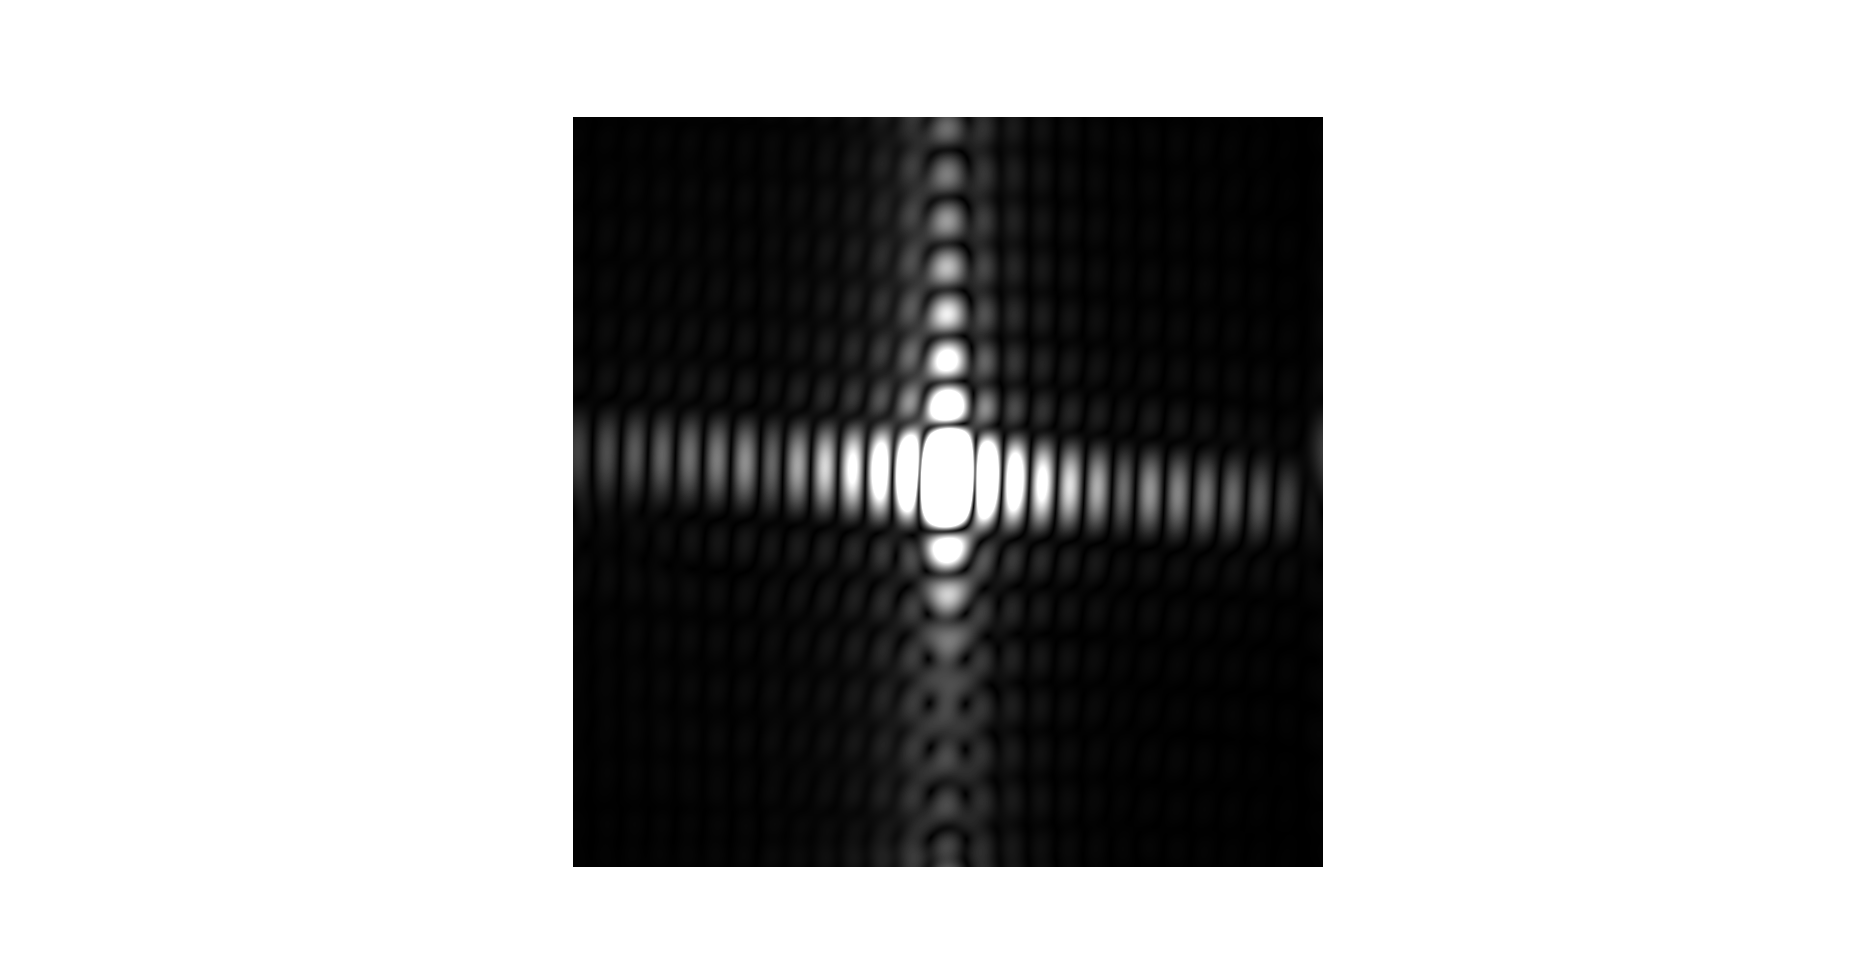
\includegraphics[width=1\textwidth]{point_target.png}
    \caption{Отклик уголкового отражателя}
    \label{fig:point_target}
\end{figure}
	
	Если мы рассчитаем волновой параметр для радиолокатора $ p = \frac{\sqrt{\lambda z}}{b} $, где $ \lambda $ - длина волны, $ z $ - наклонная дальность, $ b $ - линейный размер антенны, то он окажется намного большим 1. Это означает, что мы находимся в области диффрации Фраунгофера. Действительно, если сравнить диффракционную картину Фраунгофера на прямоугольной щели [Сивухин](рисунок \ref{fig:sivukhin}), с изображением отклика от точечной цели (рисунок \ref{fig:point_target}), то можно предположить, что механизм формироания отклика от уголкового отражателя схож с механизмом формировния диффракции, что по сути является проявлением волновой природы света.

\begin{figure}[ht]
    \centering
    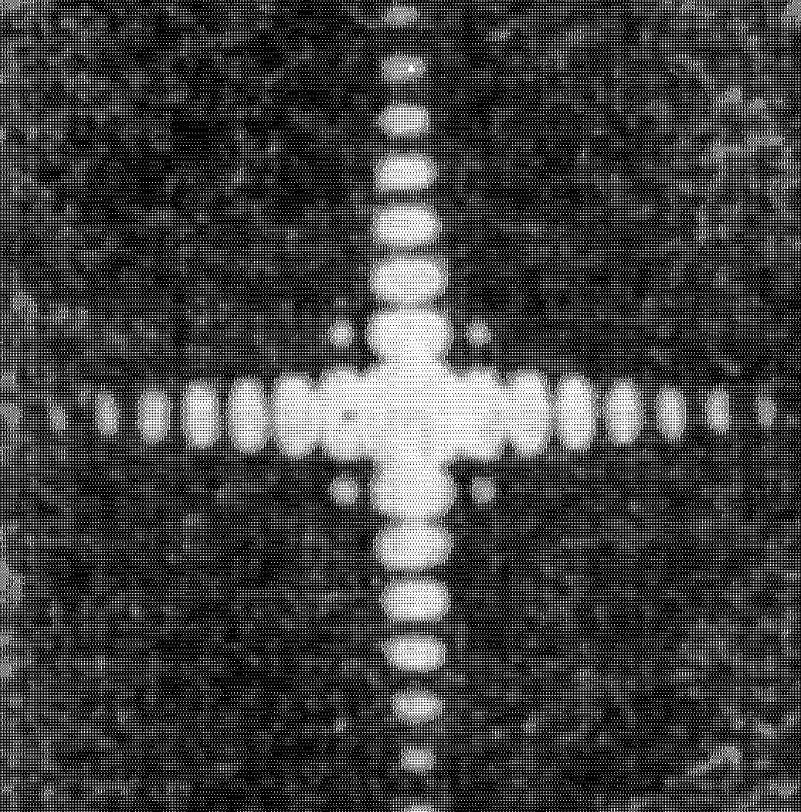
\includegraphics[width=0.4\textwidth]{sivukhin.png}
    \caption{Диффракция Фраунгофера на прямоуголной щели}
    \label{fig:sivukhin}
\end{figure}
	
	Таким образом, можно предположить, что диффракция может происходить не только на уголковых отражателях, но и на других искусственных объектах. Действительно, если взглянуть на РЛИ зданий или кораблей на рисунке \ref{fig:ship_build}, то можно в этом убедиться.
	
\begin{figure}[ht]
    \centering
    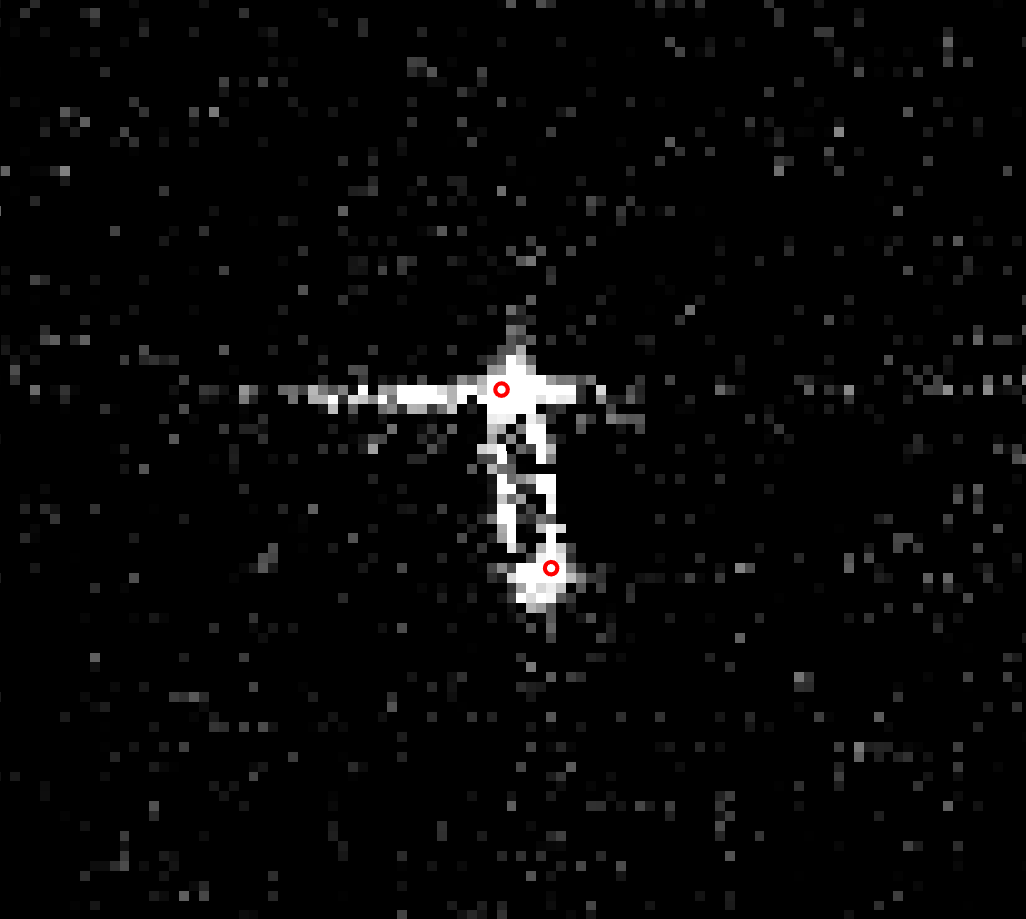
\includegraphics[width=0.4\textwidth]{ship.png}
    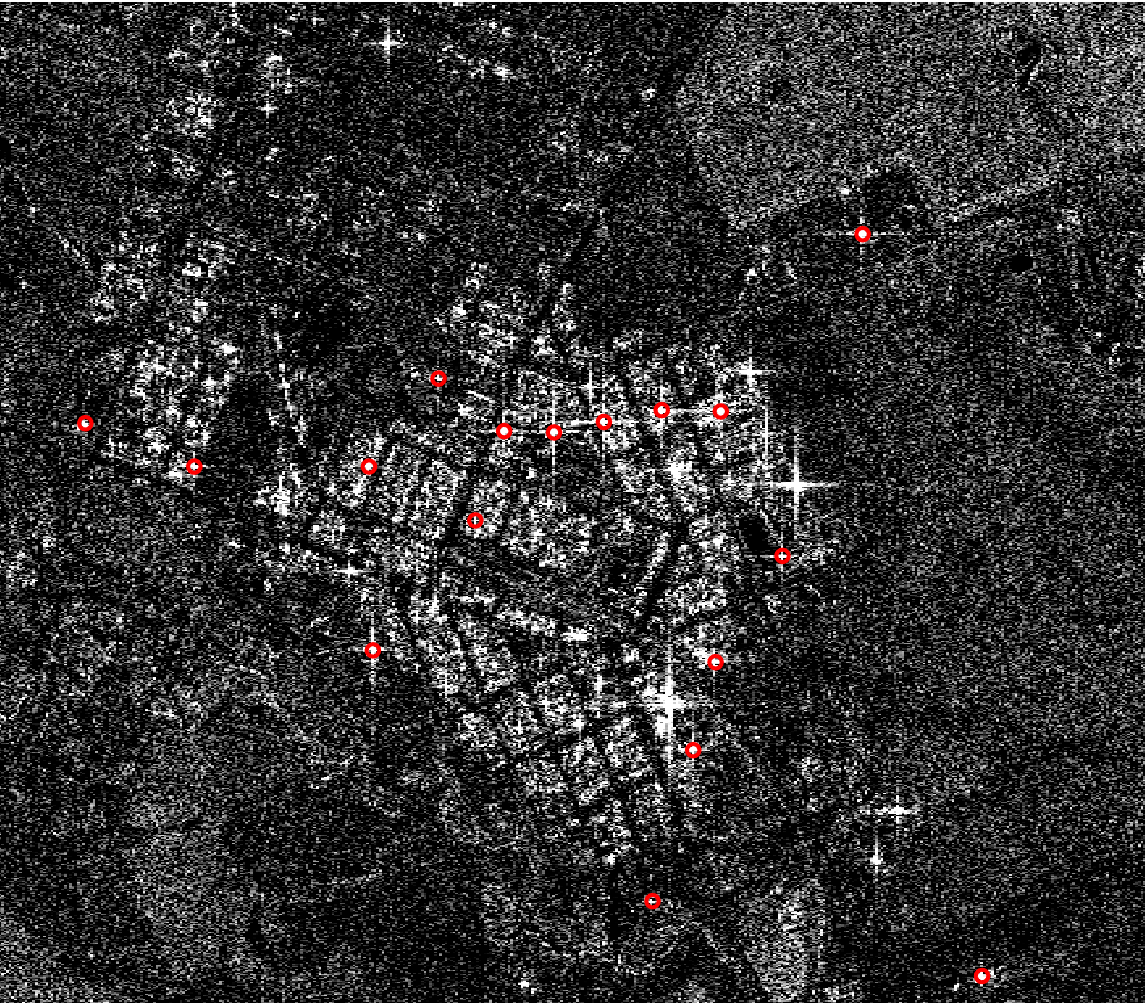
\includegraphics[width=0.4\textwidth]{building.png}
    \caption{РЛИ корабля и зданий}
    \label{fig:ship_build}
\end{figure}
		
	Проблема диффракции на произвольных искусственных объектах заключается в том, что они не являются одиночными, изолированными рассеивателями, то есть не являются точечным целями. По умолчанию отклик от таких объектов будет суммой откликов от точечных целей. И в виду ограниченной разрешающей спсобности радиолокатора они будут сливаться в единую диффракционую картину. Такие объекты, для которых нельзя с полной уверенностью сказать, что они являются одиночными, изолированным рассеивателями, но в тоже время сохраняют диффракционную картину, в данной работе будут называться псевдоточечными целями. 

	Исходя из цели исследования задача данной работы сводится к разработке алгоритма автоматического контроля качества синтеза РЛИ, используя метод анализа отклика от псевдоточечных целей, при отсутствии априорной инфомации о снимаемой сцене. Эффективность разработанного алгоритма будет определятся тем, насколько полученные значения будут отличаться от значений, полученных с помощью точечных целей.

	Таким образом задачи формулируются следующим образом:
	
	1. Разработать алгоритм автоматического поиска псевдоточечных целей на РЛИ
	
	2. Разработать алгоритм анализа отклика от псевдоточечных целей

\newpage
